\documentclass[tikz,border=4pt]{standalone}
\usepackage{tikz}
\usepackage{amsmath}
\usetikzlibrary{arrows.meta,calc,positioning,shapes.geometric,shapes.misc,
                backgrounds,fit,decorations.markings}

\begin{document}
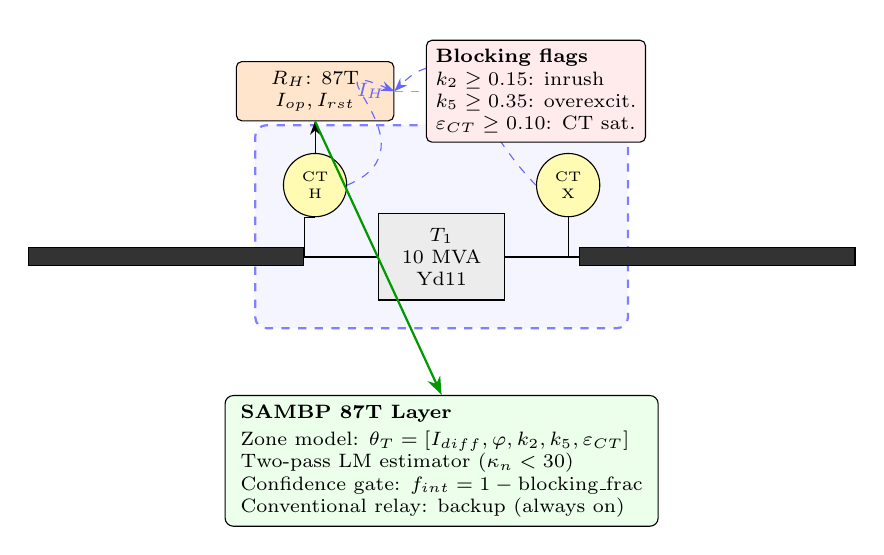
\begin{tikzpicture}[
  font=\small,
  >=Stealth,
  bus/.style     ={draw,fill=black!80,minimum width=3.5cm,minimum height=0.12cm},
  xfmr/.style    ={draw,rectangle,minimum width=1.6cm,minimum height=1.1cm,
                   fill=gray!15,align=center,font=\scriptsize},
  ct/.style      ={draw,circle,minimum size=0.55cm,fill=yellow!30,
                   font=\tiny,align=center},
  relay/.style   ={draw,rectangle,minimum width=2.0cm,minimum height=0.7cm,
                   fill=orange!20,align=center,font=\scriptsize,rounded corners=2pt},
  zone/.style    ={draw=blue!50,dashed,thick,rounded corners=4pt,
                   fill=blue!4,inner sep=6pt},
  label/.style   ={font=\scriptsize\itshape},
]

%% ============================================================
%%  HV bus (left) and LV bus (right)
%% ============================================================
\node[bus,label=above:\textbf{HV Bus (33 kV)}] (hvbus) at (0,0) {};
\node[bus,label=above:\textbf{LV Bus (11 kV)}] (lvbus) at (7,0) {};

%% ============================================================
%%  Transformer body
%% ============================================================
\node[xfmr] (xfmr) at (3.5, 0)
      {\textbf{$T_1$}\\10 MVA\\Yd11};

%% Connection HV bus → transformer
\draw[thick] (hvbus.east) -- (xfmr.west);
%% Connection transformer → LV bus
\draw[thick] (xfmr.east)  -- (lvbus.west);

%% ============================================================
%%  HV CT + relay
%% ============================================================
\node[ct,above=0.5cm of xfmr.west,xshift=-0.8cm] (ctH) {CT\\H};
\node[relay,above=0.4cm of ctH] (relayH)
      {$R_H$: 87T\\$I_{op},I_{rst}$};
\draw[->] (ctH.north) -- (relayH.south);
\draw ($(hvbus.east)+(0,0)$) -- ++(0,0.5) -| (ctH.south);

%% ============================================================
%%  LV CT + relay
%% ============================================================
\node[ct,above=0.5cm of xfmr.east,xshift=0.8cm] (ctX) {CT\\X};
\draw (ctX.south) |- ($(xfmr.east)+(0.4,0)$);

%% Both CTs feed the differential relay
\draw[->,dashed,blue!60] (ctH.east) .. controls +(1.2,0.5) and +(-1.2,0.5)
      .. node[above,font=\scriptsize]{$I_H$} (relayH.east);
\draw[->,dashed,blue!60] (ctX.west) .. controls +(-0.8,0.8) and +(0.8,0.8)
      .. node[above,font=\scriptsize]{$I_X$} (relayH.east);

%% ============================================================
%%  Zone boundary
%% ============================================================
\begin{scope}[on background layer]
  \node[zone,fit=(xfmr)(ctH)(ctX),inner sep=10pt,
        label={[font=\scriptsize\bfseries,blue!70]above:Protected Zone}] {};
\end{scope}

%% ============================================================
%%  SAMBP block
%% ============================================================
\node[draw,fill=green!8,rounded corners=3pt,
      below=1.2cm of xfmr,align=left,font=\scriptsize,
      minimum width=5.5cm] (sambp)
      {\textbf{SAMBP 87T Layer}\\[2pt]
       Zone model: $\theta_T=[I_{diff},\varphi,k_2,k_5,\varepsilon_{CT}]$\\
       Two-pass LM estimator ($\kappa_n < 30$)\\
       Confidence gate: $f_{int}=1-\text{blocking\_frac}$\\
       Conventional relay: backup (always on)};

\draw[->,thick,green!60!black] (relayH.south) -- (sambp.north);

%% ============================================================
%%  Annotation: blocking flags
%% ============================================================
\node[draw,fill=red!8,rounded corners=2pt,
      right=0.4cm of relayH,align=left,font=\scriptsize,
      minimum width=2.6cm] (flags)
      {\textbf{Blocking flags}\\
       $k_2 \geq 0.15$: inrush\\
       $k_5 \geq 0.35$: overexcit.\\
       $\varepsilon_{CT}\geq 0.10$: CT sat.};
\draw[dashed,gray!70] (relayH.east) -- (flags.west);

\end{tikzpicture}
\end{document}
